\section{Figuras de resultados}

\subsection{Prueba 1: L\'inea base (20 dispositivos)}

\begin{figure}[!t]
    \centering
    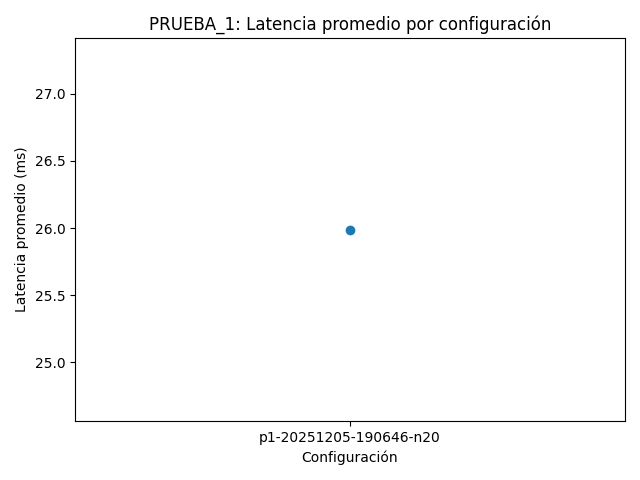
\includegraphics[width=0.8\linewidth]{resultados/figuras_auto/prueba_1_latencia.png}
    \caption{Prueba 1: Latencia promedio con 20 dispositivos.}
\end{figure}

\begin{figure}[!t]
    \centering
    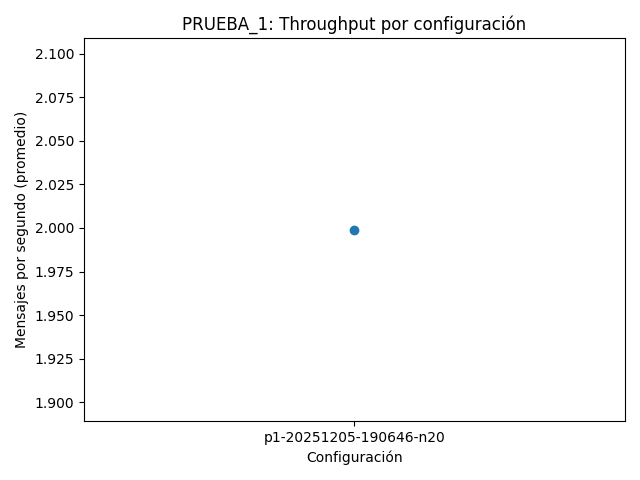
\includegraphics[width=0.8\linewidth]{resultados/figuras_auto/prueba_1_throughput.png}
    \caption{Prueba 1: Throughput agregado con 20 dispositivos.}
\end{figure}

% --------------------------------------------------------------

\subsection{Prueba 2: Escalamiento del n\'umero de dispositivos}

\begin{figure}[!t]
    \centering
    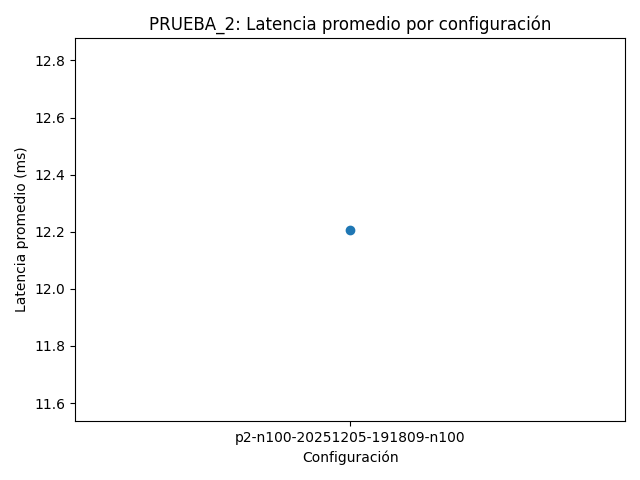
\includegraphics[width=0.8\linewidth]{resultados/figuras_auto/prueba_2_latencia.png}
    \caption{Prueba 2: Latencia promedio para \{50, 100, 200, 400\} dispositivos.}
\end{figure}

\begin{figure}[!t]
    \centering
    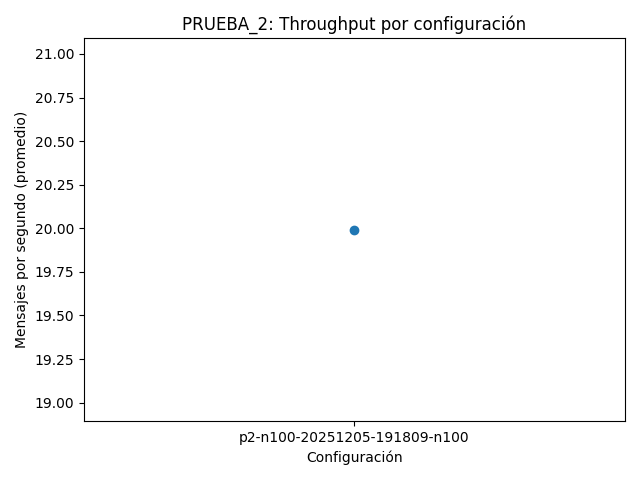
\includegraphics[width=0.8\linewidth]{resultados/figuras_auto/prueba_2_throughput.png}
    \caption{Prueba 2: Throughput total en funci\'on del n\'umero de dispositivos.}
\end{figure}

% --------------------------------------------------------------

\subsection{Prueba 3: Variaci\'on del intervalo de env\'io}

\begin{figure}[!t]
    \centering
    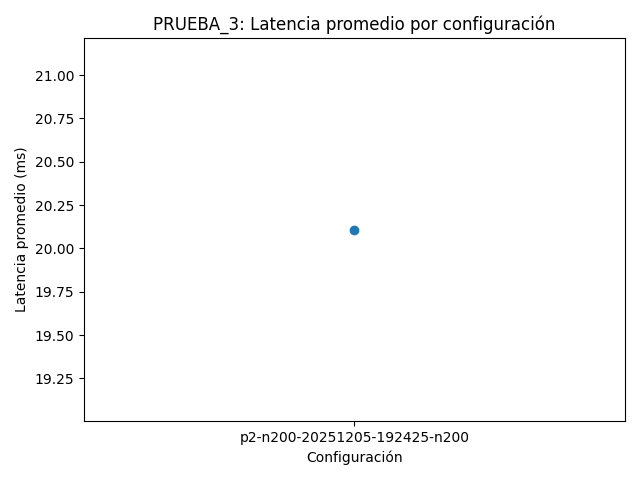
\includegraphics[width=0.8\linewidth]{resultados/figuras_auto/prueba_3_latencia.png}
    \caption{Prueba 3: Latencia promedio para intervalos de \{10s, 5s, 2s, 1s\}.}
\end{figure}

\begin{figure}[!t]
    \centering
    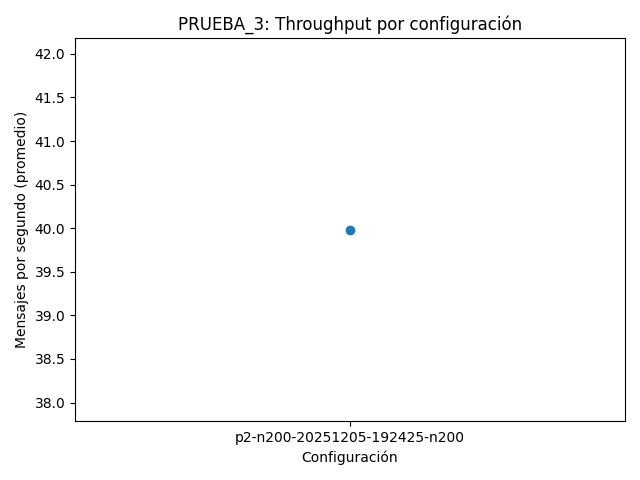
\includegraphics[width=0.8\linewidth]{resultados/figuras_auto/prueba_3_throughput.png}
    \caption{Prueba 3: Throughput alcanzado seg\'un el intervalo de env\'io.}
\end{figure}

% --------------------------------------------------------------

\subsection{Prueba 4: Tama\~no del payload}

\begin{figure}[!t]
    \centering
    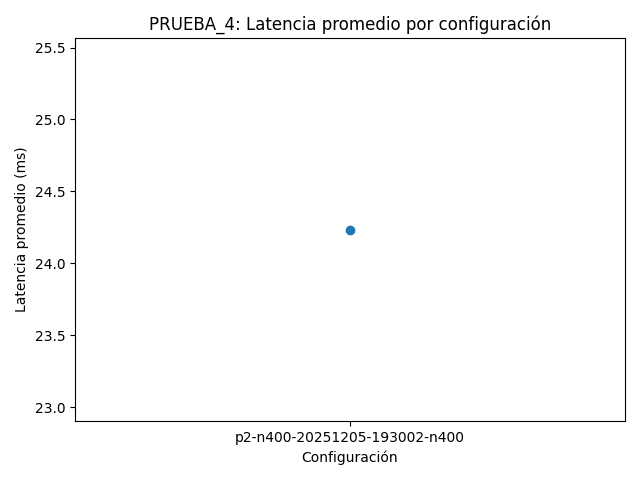
\includegraphics[width=0.8\linewidth]{resultados/figuras_auto/prueba_4_latencia.png}
    \caption{Prueba 4: Latencia promedio seg\'un tama\~no del payload (small, medium, large).}
\end{figure}

\begin{figure}[!t]
    \centering
    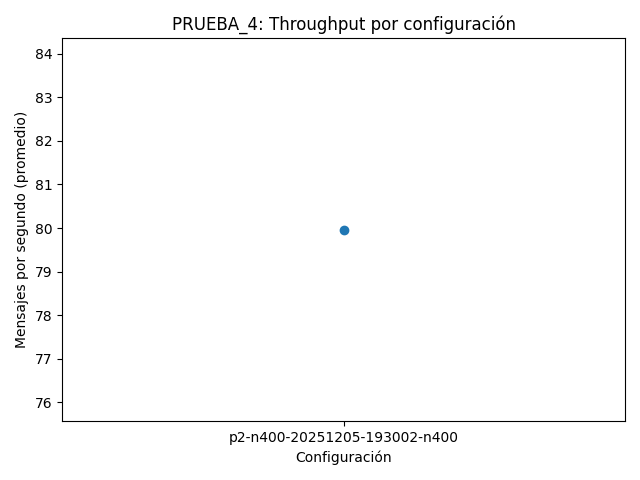
\includegraphics[width=0.8\linewidth]{resultados/figuras_auto/prueba_4_throughput.png}
    \caption{Prueba 4: Throughput para cada tama\~no de payload con 200 dispositivos.}
\end{figure}

% --------------------------------------------------------------

\subsection{Prueba 5: Rate limit vs env\'io directo}

\begin{figure}[!t]
    \centering
    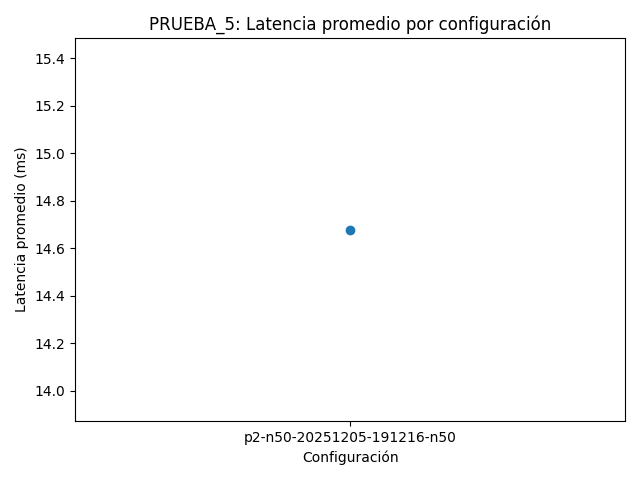
\includegraphics[width=0.8\linewidth]{resultados/figuras_auto/prueba_5_latencia.png}
    \caption{Prueba 5: Latencia promedio entre modos sin agregaci\'on vs con rate limit.}
\end{figure}

\begin{figure}[!t]
    \centering
    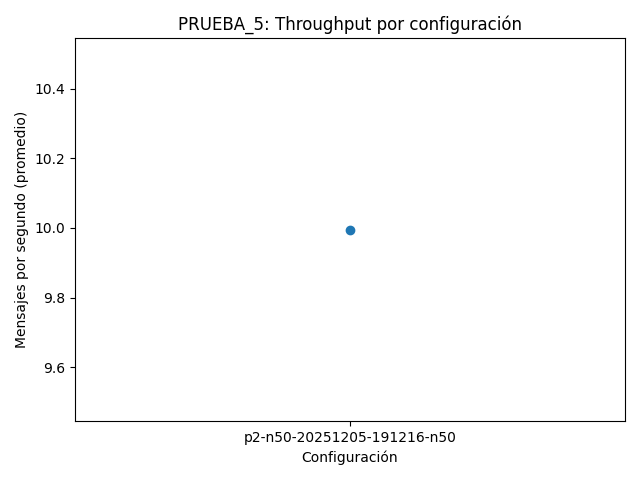
\includegraphics[width=0.8\linewidth]{resultados/figuras_auto/prueba_5_throughput.png}
    \caption{Prueba 5: Throughput comparativo entre ambos modos.}
\end{figure}

% --------------------------------------------------------------

\subsection{Prueba 6: Escenario as\'incrono}

\begin{figure}[!t]
    \centering
    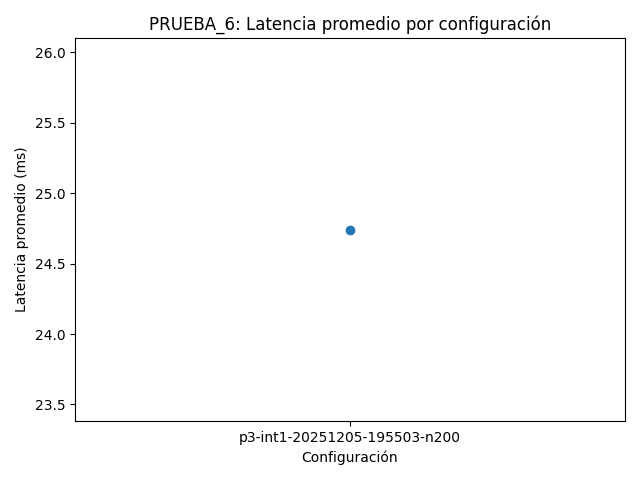
\includegraphics[width=0.8\linewidth]{resultados/figuras_auto/prueba_6_latencia.png}
    \caption{Prueba 6: Latencia promedio para configuraciones as\'incronas.}
\end{figure}

\begin{figure}[!t]
    \centering
    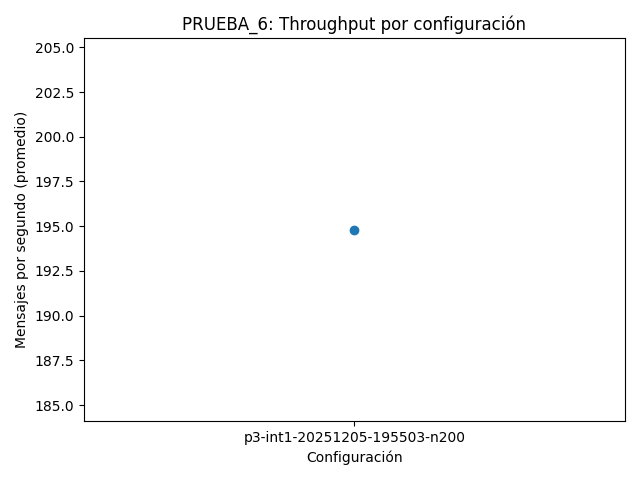
\includegraphics[width=0.8\linewidth]{resultados/figuras_auto/prueba_6_throughput.png}
    \caption{Prueba 6: Throughput total bajo ejecuci\'on as\'incrona.}
\end{figure}
